
\begin{task}{5, Tests}

\paragraph{TEST 4 - RiMEA scenario 7: demographic parameters}

The RiMEA scenario 7. demographic parameters, we focus on having different walking speeds for different pedestrians depending on their demographics.\\ There are 50 pedestrians in total, and we will assign the different speeds for the specific group according to their individual conditions, 10 pedestrians as a group. 

The various speeds are sampled from a specific interval that depends on the age and moving ability of the group(in our project, we have the speed range from 0 to 1). The group are assigned in the following way:
\begin{itemize}
    \item 3-10 years old: speed $\in[0.1, 0.2)$ m/s
    \item 10-18 years old: speed $\in[0.3, 0.45)$ m/s
    \item 18-50 years old: speed $\in[0.76, 0.85)$ m/s
    \item 51-80 years old: speed $\in[0.2, 0.45)$ m/s
    \item Persons with impaired mobility: speed $\in[0.46, 0.76)$ m/s
\end{itemize}
We have grouped the people with their ages from the youngest 3 to the oldest 80, and also include disabled people as a part of the consideration. We set the Grid table with the size is 80 x 80. Iteration time is 100. And all the pedestrians with initialized speeds according to their age, The red vertical line on the figure below shows that all the pedestrians start from the left with the same distance to reach the target. The target is also aligned vertically on the right of the figure. The gap between the target is just to check if the target does not match the pedestrian, and how the trajectory looks like. 
\begin{figure}[H] 
\centering
\subfigure[Start Position]{
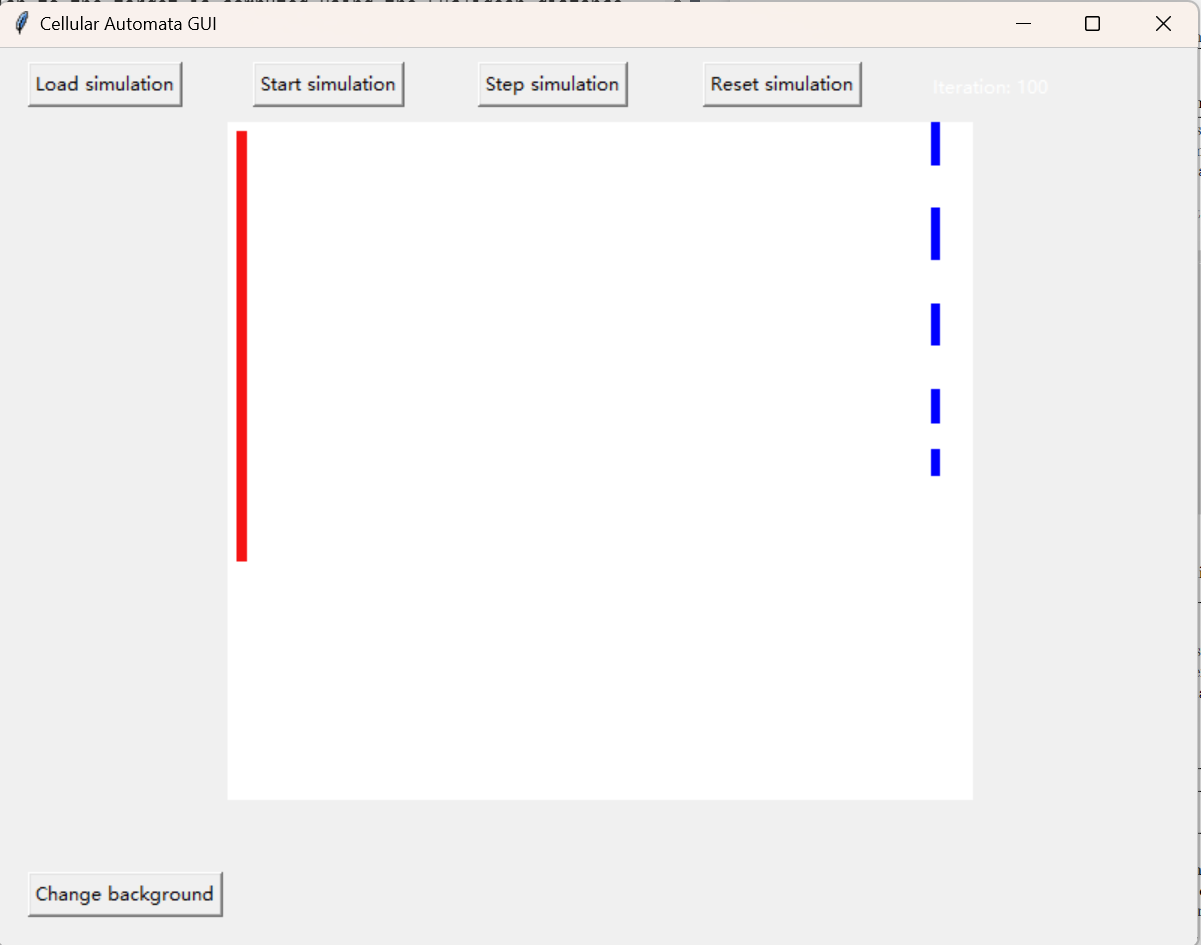
\includegraphics[width=0.4\textwidth]{report-template/image/Task5-sec7.png}}
\subfigure[The mid position]{
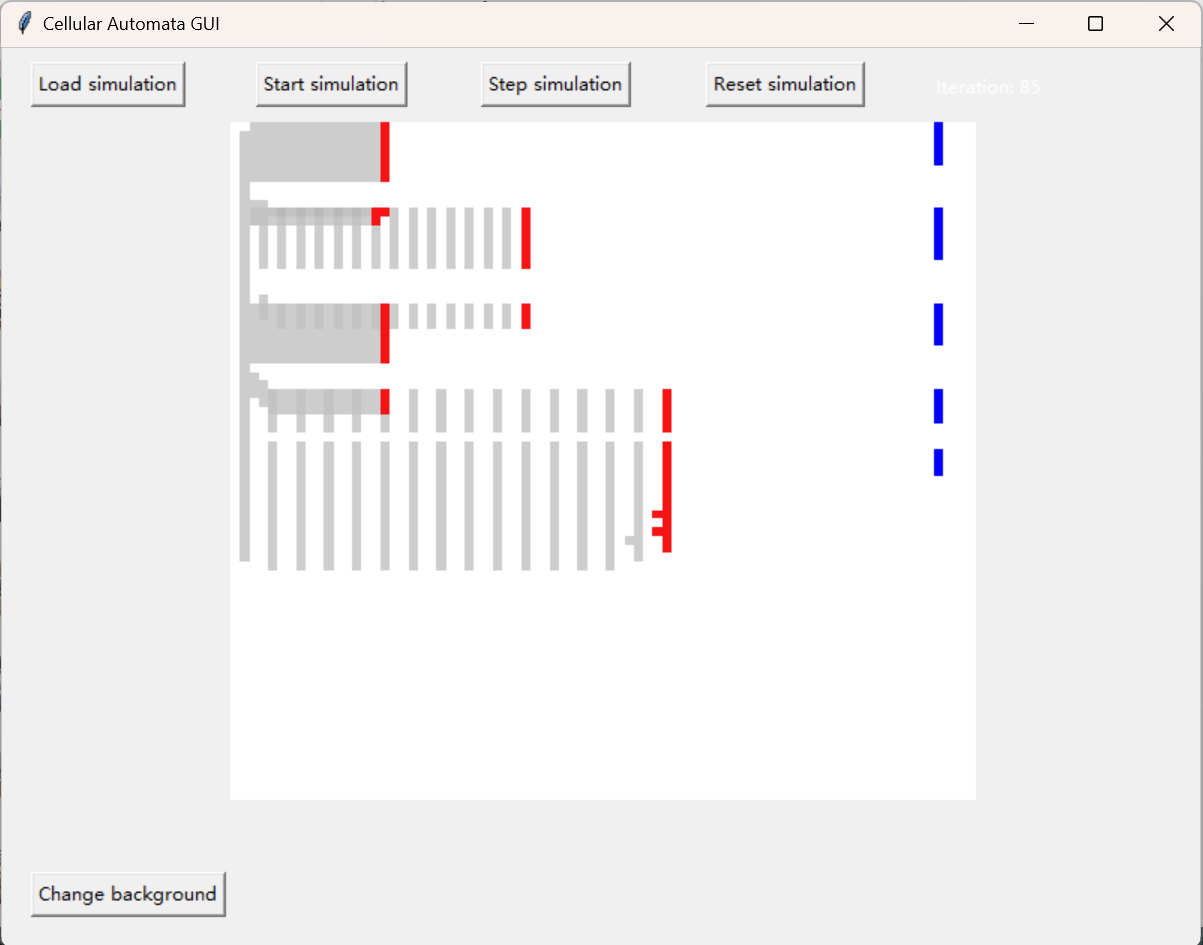
\includegraphics[width=0.4\textwidth]{report-template/image/Task5-sec7.1.png}}
\subfigure[The unfinished simulation]{
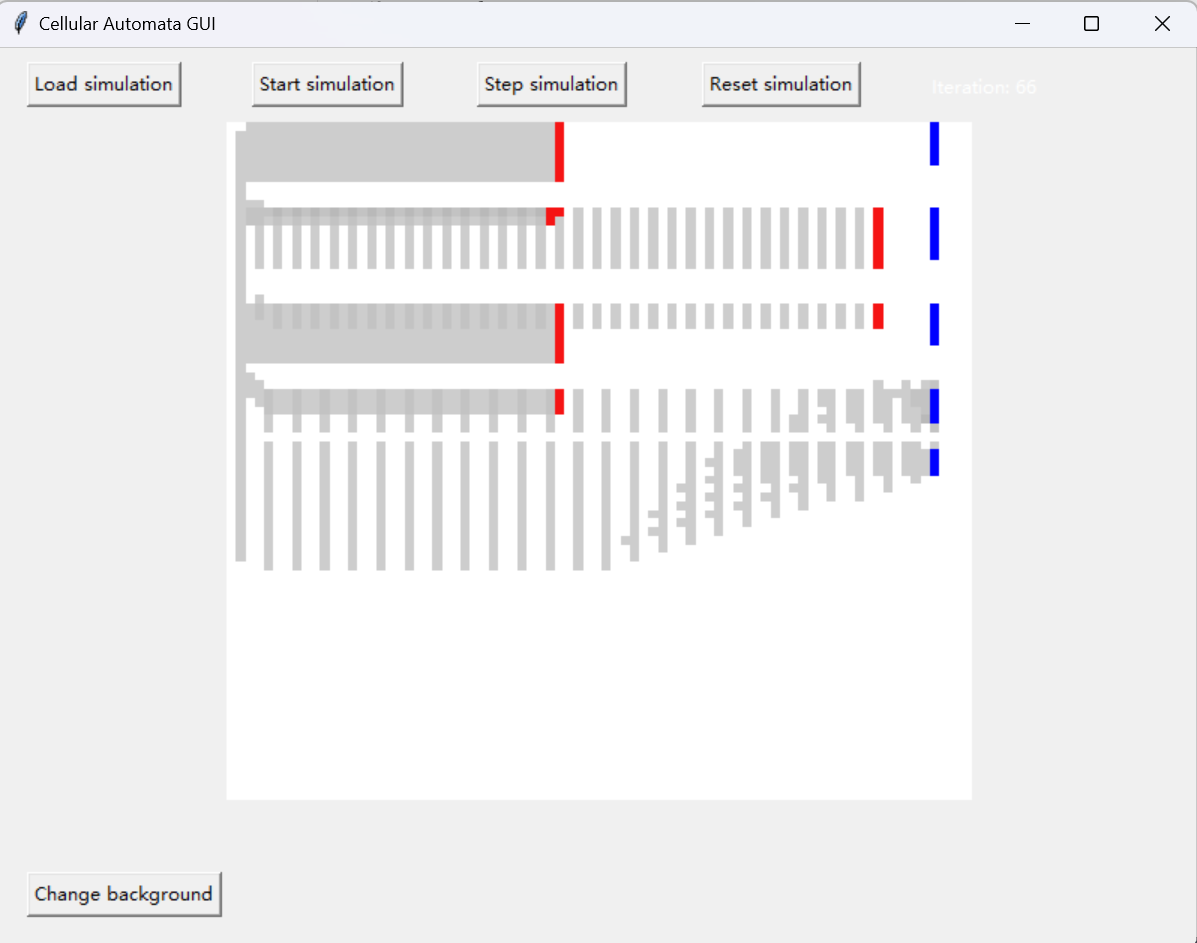
\includegraphics[width=0.4\textwidth]{report-template/image/Task5-sec7.2.png}}
\subfigure[end position]{
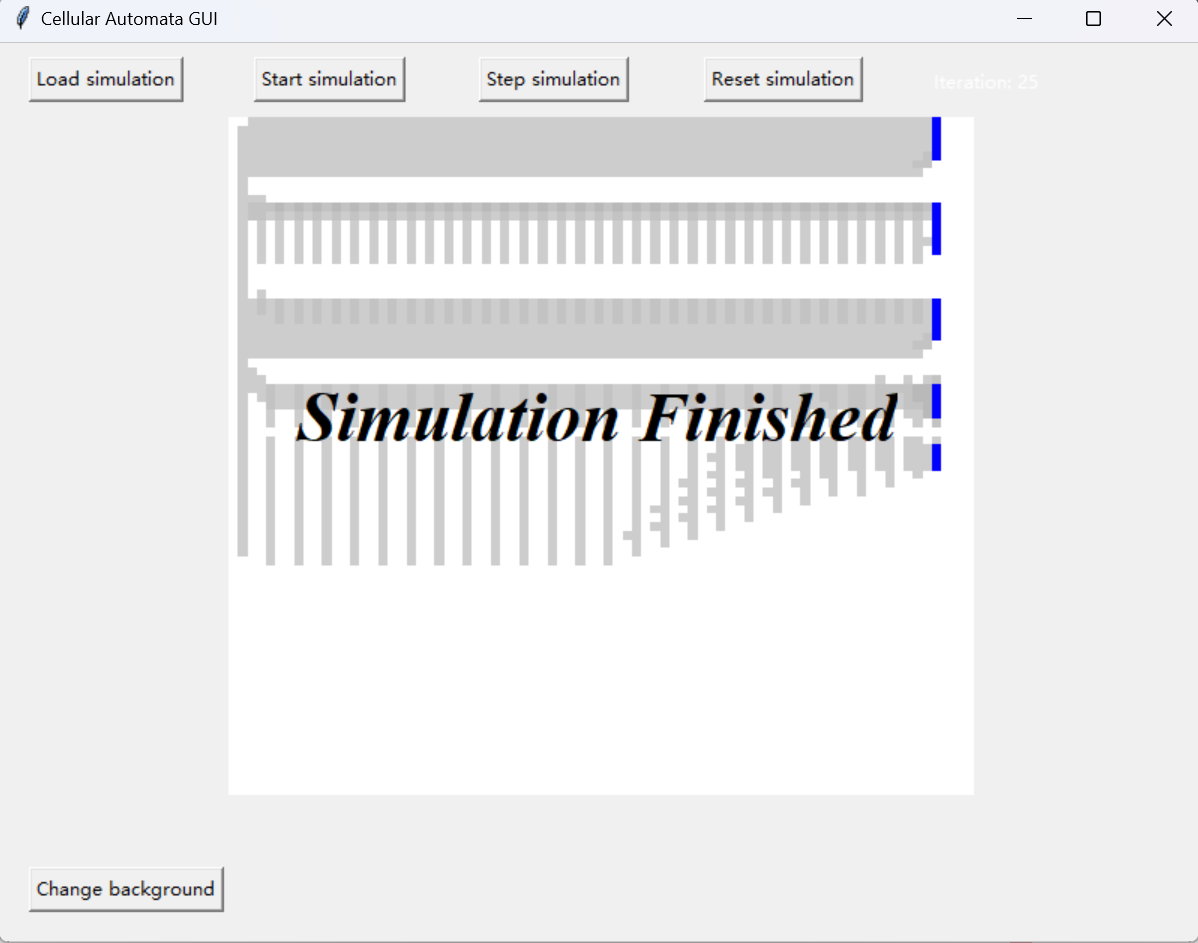
\includegraphics[width=0.4\textwidth]{report-template/image/Task5-sec7.3.png}}
\caption{RIMEA scenario-7}
\end{figure}
As we can see the pedestrians are not moving together but at their own speed which is assigned by their age or health condition. The first group is aged 10 to 18. The second is disabled, the Third is aged 3-10, The fourth and fifth are 18 to 50. Speed is the main effect of the pedestrian movement. Obviously, the higher speed moves faster than the lower speed. cause the spaces are all the same under this experiment condition the space(the distance between the pedestrians and targets is 75) and it comes with a fixed running time. Pressing the start simulation button, the simulation will automatically run until the runs out of the iterations. Continuously clicking the step simulation will make the rest pedestrians arrive at the target.
\end{task}